\documentclass[12pt,a4paper]{article}
\renewcommand{\baselinestretch}{1.5}
\usepackage[latin1]{inputenc}
\usepackage{amsmath}
\usepackage{amsfonts}
\usepackage{amssymb}
\usepackage{algorithm}
\usepackage{algpseudocode}
\usepackage{graphicx}
\usepackage{geometry}
\usepackage{tabulary}
\usepackage{caption}
\usepackage{subcaption}
\usepackage{xcolor}
\usepackage{bm}
\usepackage{longtable}
\usepackage{booktabs}
\usepackage{tikz}
\usetikzlibrary{positioning,arrows.meta}

\usepackage{comment}
\usepackage[hyphens]{url}
\graphicspath{{./results/}}

\geometry{
    left=2.5cm,
    right=2.5cm,
    top=2.5cm,
    bottom=3cm,
}

\usepackage{titlesec}
\setcounter{secnumdepth}{4}
\setcounter{tocdepth}{4}
\titleformat{\paragraph}
{\normalfont\normalsize\bfseries}{\theparagraph}{1em}{}
\titlespacing*{\paragraph}
{0pt}{3.25ex plus 1ex minus .2ex}{1.5ex plus .2ex}

\newenvironment{conditions}
{\par\vspace{\abovedisplayskip}\noindent\begin{tabular}{>{$}l<{$} @{${}={}$} l}}{\end{tabular}\par\vspace{\belowdisplayskip}}

\begin{document}

    \input{titlepage}

    \pagenumbering{gobble}
    \renewcommand*\contentsname{Table of Contents}
    \tableofcontents
    \newpage
    \newpage
    \listoffigures
    \newpage
    \newpage
    \listoftables
    \newpage
    \pagenumbering{arabic}

%% ===========================================================================
\section{Introduction}
%% ===========================================================================

\subsection{Background}

The rapid growth of scientific computing, computer graphics, and data-driven
simulation has created an immense demand for algorithms that can process large
two-dimensional spatial domains efficiently.  One fundamental problem in this
space is computing a \textit{Centroidal Voronoi Tessellation} (CVT), wherein a
set of $N$ generator sites partitions a domain into regions such that each site
coincides with the density-weighted centroid of its own region
\cite{du1999centroidal}.  CVTs are widely used in mesh generation, image
stippling, point-cloud simplification, and adaptive sampling for physics
simulations.

The classical solver for CVT is \textit{Lloyd's algorithm} \cite{lloyd1982least},
an iterative fixed-point method that alternates between two steps:
\begin{itemize}
    \item \textbf{Assignment:} label every grid pixel with the index of its
          nearest site.
    \item \textbf{Update:} move each site to the density-weighted centroid of its
          labeled region.
\end{itemize}
On a grid of $P = W \times H$ pixels with $N$ sites, the brute-force assignment
step costs $O(P \cdot N)$ per iteration --- prohibitively slow for the large
grids and tight convergence tolerances demanded by modern applications.

Graphics Processing Units (GPUs) offer a compelling solution.  An NVIDIA RTX
2050 (Ampere GA107, sm\_86) provides 2048 CUDA cores and 4~GB of GDDR6 memory,
delivering a theoretical peak throughput several orders of magnitude higher than
a contemporary CPU \cite{kirk2022programming}.  However, achieving that peak
requires careful algorithm design: the memory subsystem, warp occupancy, and
PCIe transfer cost all become critical factors that must be understood and
optimised.

\subsection{Introduction to Problem Statement}

This project investigates the end-to-end GPU acceleration of Density-Weighted
CVT on an NVIDIA RTX 2050 laptop GPU.  Specifically, it addresses three
engineering challenges that prevent naive GPU ports from reaching peak
performance:

\begin{itemize}
    \item \textbf{Algorithmic complexity:} brute-force Voronoi assignment is
          $O(P \cdot N)$; the Jump Flooding Algorithm (JFA) \cite{rong2006jump}
          reduces this to $O(P \log P)$ using a ping-pong propagation scheme.
    \item \textbf{Memory contention:} accumulating density-weighted centroids
          requires summing millions of per-pixel contributions into $N$ shared
          accumulators.  Unguarded global \texttt{atomicAdd} calls saturate DRAM
          bandwidth; block-local shared-memory staging reduces global atomic
          traffic by a factor equal to the block size.
    \item \textbf{PCIe overhead and launch configuration:} the cost of
          transferring the density grid, site positions, and the final assignment
          array over the 16~GB/s PCIe~3.0 bus is non-negligible for small
          problem sizes, creating a \textit{crossover point} below which the CPU
          serial implementation is faster.  The choice of CUDA thread-block size
          also affects warp occupancy and kernel throughput.
\end{itemize}

Figure~\ref{fig:cuda-512} shows an example CVT output produced by the CUDA
backend on a $512 \times 512$ Gaussian density field with 256 sites after 100
Lloyd iterations.

\begin{figure}[h!]
    \centering
    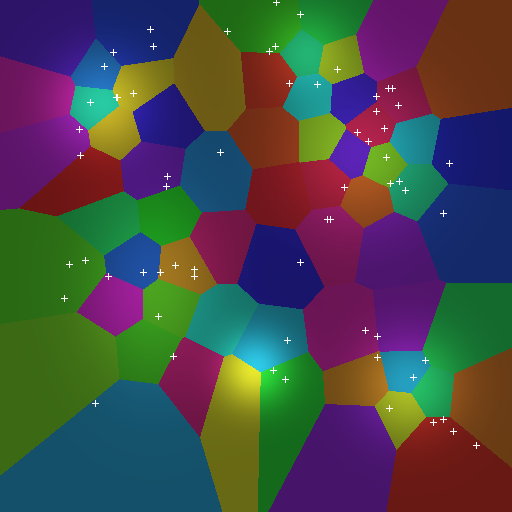
\includegraphics[width=0.65\linewidth]{cuda_512x512}
    \caption{CVT result: 256 sites on a $512\times512$ Gaussian density field
             (CUDA backend, 100 iterations).  Brighter regions receive more
             sites due to higher density weighting.}
    \label{fig:cuda-512}
\end{figure}

%% ===========================================================================
\newpage
\section{Literature Review}
%% ===========================================================================

Table~\ref{tab:litreview} summarises the key prior work that motivates the
design decisions in this project.

\begin{longtable}{|p{2.5cm}|p{3.0cm}|p{3.0cm}|p{3.3cm}|p{3.3cm}|}
\caption{Summary of Literature Review}
\label{tab:litreview}\\
\hline
\textbf{Reference} &
\textbf{Concepts Highlighted} &
\textbf{Technique(s) Used} &
\textbf{Significance / Proposal} &
\textbf{Limitations} \\
\hline
\endfirsthead
\hline
\textbf{Reference} &
\textbf{Concepts Highlighted} &
\textbf{Technique(s) Used} &
\textbf{Significance / Proposal} &
\textbf{Limitations} \\
\hline
\endhead

\cite{du1999centroidal} &
Centroidal Voronoi Tessellation; density-weighted partitioning &
Lloyd's iterative algorithm;
Monte-Carlo sampling &
Establishes CVT as a rigorous mathematical framework for optimal
site placement in a weighted domain &
Purely theoretical analysis; no GPU implementation; $O(P \cdot N)$
assignment cost limits scalability \\
\hline

\cite{lloyd1982least} &
Vector quantisation; least-squares centroidal partitioning &
Fixed-point iteration on Voronoi assignment and centroid update &
Foundational algorithm underlying virtually all CVT implementations;
easy to parallelise at the pixel level &
Convergence is slow (many iterations); brute-force distance queries
scale poorly with both $N$ and $P$ \\
\hline

\cite{rong2006jump} &
GPU-accelerated Voronoi diagram; Jump Flooding Algorithm (JFA) &
Iterative ping-pong propagation at decreasing strides $\{2^{k},\dots,1\}$ &
Reduces Voronoi assignment from $O(P \cdot N)$ to $O(P \log P)$,
enabling real-time computation on large textures &
Small residual errors near Voronoi boundaries; requires two
ping-pong buffers doubling device memory usage \\
\hline

\cite{kirk2022programming} &
CUDA memory hierarchy; warp occupancy; shared-memory optimisation &
Hardware-aware kernel design; occupancy analysis via \texttt{cudaOccupancy} API &
Provides the theoretical foundation for shared-memory staging and
launch-configuration tuning used in this project &
Textbook-level treatment; specific RTX 2050 (Ampere sm\_86)
characteristics require empirical measurement \\
\hline

\cite{nvidia2023cuda} &
PCIe transfer cost; pinned memory; CUDA Event timing &
\texttt{cudaMallocHost} for pinned buffers;
\texttt{cudaEventRecord/ElapsedTime} for precise kernel timing &
Defines the measurement methodology used in all benchmarks in
this project; establishes baseline transfer bandwidth of PCIe 3.0 &
Documentation only; no application-specific crossover analysis for
CVT workloads \\
\hline

\cite{nvidia2020ampere} &
NVIDIA Ampere GA102 architecture; sm\_86 warp scheduler; SM occupancy model &
Architecture whitepaper (specification-level data) &
Direct source for sm\_86 properties (48 warps/SM, 128 CUDA cores/SM, 4\,GB GDDR6)
used to interpret occupancy measurements in Table~\ref{tab:blocksize} &
Architectural description only; no performance model for
memory-bound CVT workloads \\
\hline

\cite{openmp2021} &
Fork-join threading model; work-sharing constructs; \texttt{schedule} clauses &
\texttt{\#pragma omp parallel for} with static scheduling &
Baseline multi-core backend; provides the serial-to-OMP speedup baseline
($7\times$ on 12 logical cores) against which CUDA is evaluated &
Shared-memory only; no GPU offload; Amdahl overhead limits efficiency
to $\approx$58\% at 12 threads \\
\hline

\cite{amdahl1967validity} &
Parallel speedup ceiling; serial fraction bottleneck &
Analytical speedup bound $S \leq 1/(f + (1-f)/N)$ &
Explains the sub-linear OMP efficiency observed in Table~\ref{tab:speedup};
serial centroid-update fraction limits OpenMP to $\approx$7$\times$ &
Ignores memory-bandwidth saturation, which further limits
observed OMP speedup to below Amdahl prediction \\
\hline

\cite{harris2007optimizing} &
CUDA parallel reduction; shared-memory staged accumulation &
Two-phase reduction: block-local shmem then global atomic &
Directly motivates the shared-memory centroid accumulation kernel
(Algorithm~\ref{alg:centroid}); reduces global \texttt{atomicAdd} calls
by a factor of blockDim.x &
Reduction strategy assumes uniform data; density-weighted CVT
centroids require per-pixel weight scaling before accumulation \\
\hline
\end{longtable}


%% ===========================================================================
\section{Research Gaps}
%% ===========================================================================

Based on the literature review, the following gaps motivate the present work:

\begin{itemize}
    \item \textbf{Lack of end-to-end GPU CVT benchmarks:}  Prior work
          \cite{rong2006jump} demonstrates JFA in isolation (Voronoi diagram
          generation) but does not integrate it into a full Lloyd-iteration CVT
          solver with density weighting, shared-memory centroid accumulation,
          and convergence tracking on modern Ampere hardware.

    \item \textbf{Ignored PCIe crossover effects:}  Theoretical complexity
          analyses (\cite{du1999centroidal}, \cite{lloyd1982least}) compare
          algorithmic complexity but ignore the fixed PCIe data-transfer latency
          that makes GPU solutions \textit{slower} than CPU solutions for small
          problem sizes.  No study has quantified this crossover for CVT
          workloads.

    \item \textbf{Uncharacterised launch-configuration sensitivity:}
          The CUDA programming guide \cite{nvidia2023cuda} discusses occupancy
          generally, but the effect of block size on JFA kernel throughput for
          CVT-specific access patterns (stride-$k$ neighbour reads) has not been
          empirically profiled.
\end{itemize}

%% ===========================================================================
\newpage
\section{Problem Formulation}
%% ===========================================================================

Let $\Omega = [0,W) \times [0,H)$ be a discrete pixel grid of size
$P = W \times H$ and let $\rho : \Omega \rightarrow \mathbb{R}_{>0}$ be a
non-negative density function stored as a row-major float array.  Given $N$
initial site positions $\{s_i\}_{i=1}^{N}$ with $s_i = (x_i, y_i) \in \Omega$,
define the Voronoi cell of site $i$ as:

\begin{equation}
    V_i = \{ p \in \Omega \mid \|p - s_i\|_2 < \|p - s_j\|_2 \; \forall j \neq i \}
\end{equation}

The CVT problem seeks site positions that satisfy the fixed-point condition:

\begin{equation}
    s_i^* = \frac{\displaystyle\sum_{p \in V_i} \rho(p)\, p}
                 {\displaystyle\sum_{p \in V_i} \rho(p)}
    \quad \forall\, i \in \{1,\dots,N\}
    \label{eq:centroid}
\end{equation}

Lloyd's algorithm solves Eq.~\eqref{eq:centroid} iteratively.  The
computational challenge arises from the assignment step: each of the $P$ pixels
must be compared against all $N$ sites at every iteration.  On a
$1024 \times 1024$ grid with $N = 256$ sites, this requires approximately
\mbox{$2.68 \times 10^8$} distance evaluations per iteration --- roughly
\mbox{$2.68 \times 10^{10}$} floating-point operations across 100 iterations,
far beyond the practical throughput of a serial CPU.

This project therefore formulates the following optimisation problem:
\textit{implement a CUDA GPU solver for Density-Weighted CVT that minimises
per-iteration wall-clock time subject to the constraints imposed by the PCIe
bandwidth, device memory capacity, and warp occupancy of the NVIDIA RTX 2050
(sm\_86)}.  Specifically, the implementation must:
\begin{itemize}
    \item Replace brute-force assignment with the Jump Flooding Algorithm to
          reduce per-iteration complexity from $O(P \cdot N)$ to $O(P \log P)$.
    \item Replace per-pixel global \texttt{atomicAdd} centroid accumulation with
          block-local shared-memory staging, reducing global atomic traffic by
          $\sim\!\text{blockDim.x}$ (256 times for the default block size).
    \item Characterise the PCIe bandwidth (H2D and D2H) and identify the problem
          size crossover at which GPU acceleration becomes profitable.
    \item Determine the optimal CUDA thread-block size for the JFA flood kernel
          by sweeping $\{32,64,128,256,512\}$ threads/block.
\end{itemize}

%% ===========================================================================
\section{Objectives}
%% ===========================================================================

\begin{itemize}
    \item To implement the \textbf{Jump Flooding Algorithm (JFA)} on an NVIDIA
          RTX 2050 GPU to replace brute-force Voronoi assignment and reduce
          per-iteration complexity from $O(P \cdot N)$ to $O(P \log P)$.
    \item To optimise \textbf{centroid accumulation} by replacing global
          \texttt{atomicAdd} operations with block-local shared-memory
          accumulators, reducing device-memory atomic traffic by a factor equal
          to the block size.
    \item To benchmark \textbf{PCIe transfer bandwidth} (both Host-to-Device and
          Device-to-Host) across transfer sizes from 1\,MB to 512\,MB using
          pinned memory, and to identify the \textbf{crossover problem size}
          beyond which the GPU backend outperforms the serial CPU baseline.
    \item To evaluate the sensitivity of \textbf{JFA kernel throughput} to the
          CUDA launch configuration by sweeping five thread-block sizes
          ($32, 64, 128, 256, 512$) and selecting the optimal configuration
          based on measured median kernel time and warp occupancy.
\end{itemize}

%% ===========================================================================
\newpage
\section{Methodology}
%% ===========================================================================

\subsection{System Architecture}

The solver is structured as three parallel backends sharing a common
\texttt{DensityGrid} and \texttt{RunResult} interface: a serial CPU baseline,
an OpenMP multi-core implementation, and the CUDA GPU backend studied here.
Each Lloyd iteration in the CUDA backend executes the pipeline illustrated
below:

\medskip
\noindent
\textbf{Block Diagram --- CUDA Lloyd Iteration Pipeline:}

\vspace{6pt}
\begin{figure}[h!]
\centering
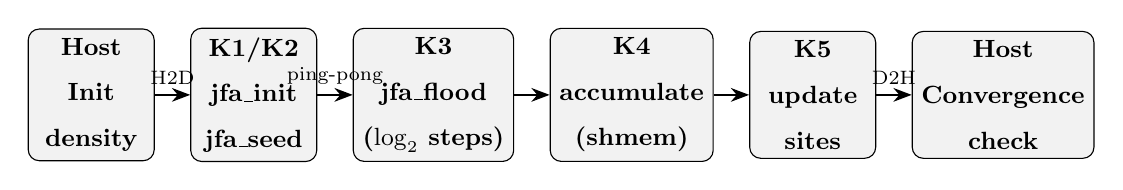
\begin{tikzpicture}[
  node distance = 1.5cm and 0.45cm,
  box/.style = {draw, rounded corners, align=center, minimum height=1.1cm,
                minimum width=1.6cm, font=\small\bfseries, fill=gray!10},
  arr/.style = {-{Stealth}, thick},
  lbl/.style = {font=\scriptsize, midway, above}
]
  \node[box] (host1) {Host\\Init\\density};
  \node[box, right=of host1] (k12)   {K1/K2\\jfa\_init\\jfa\_seed};
  \node[box, right=of k12]   (k3)    {K3\\jfa\_flood\\($\log_2$ steps)};
  \node[box, right=of k3]    (k4)    {K4\\accumulate\\(shmem)};
  \node[box, right=of k4]    (k5)    {K5\\update\\sites};
  \node[box, right=of k5]    (host2) {Host\\Convergence\\check};

  \draw[arr] (host1) -- node[lbl]{H2D} (k12);
  \draw[arr] (k12)   -- node[lbl]{ping-pong} (k3);
  \draw[arr] (k3)    -- (k4);
  \draw[arr] (k4)    -- (k5);
  \draw[arr] (k5)    -- node[lbl]{D2H} (host2);
\end{tikzpicture}
\caption{CUDA Lloyd iteration pipeline. Each iteration makes one H2D transfer
         (density grid), executes Kernels 1--5 on the GPU, then returns the
         updated site array D2H for convergence checking.}
\label{fig:pipeline}
\end{figure}
\vspace{4pt}

\subsection{Jump Flooding Algorithm (JFA)}

Algorithm~\ref{alg:jfa} describes the GPU-parallel 1+JFA variant implemented
in \texttt{jfa\_flood\_kernel}.  Each thread processes one pixel; threads
communicate only through the shared ping-pong assignment buffers.

\begin{algorithm}
\caption{GPU Jump Flooding Algorithm (1+JFA variant)}
\label{alg:jfa}
\begin{algorithmic}[1]
    \State \textbf{Input:} site positions $\{s_i\}$, grid $W \times H$
    \State \textbf{Output:} assignment buffer $A[p] = \arg\min_i \|p - s_i\|^2$
    \State Initialise $A[p] \gets -1$ for all $p$ \Comment{\texttt{jfa\_init\_kernel}}
    \State Seed $A[s_i] \gets i$ for all $i$   \Comment{\texttt{jfa\_seed\_kernel}}
    \For{$k = \lceil\log_2(\max(W,H))\rceil - 1$ \textbf{down to} $0$}
        \State stride $\gets 2^k$
        \For{each pixel $p = (px, py)$ \textnormal{[in parallel, one thread per pixel]}}
            \For{each neighbour offset $(dx, dy) \in \{-1,0,1\}^2 \setminus \{(0,0)\}$}
                \State $q \gets (px + dx \cdot \text{stride},\; py + dy \cdot \text{stride})$
                \If{$q$ is in-bounds and $A[q] \neq -1$}
                    \If{$\|p - s_{A[q]}\|^2 < \|p - s_{A[p]}\|^2$}
                        \State $A[p] \gets A[q]$
                    \EndIf
                \EndIf
            \EndFor
        \EndFor
        \State swap ping-pong buffers
    \EndFor
    \State Repeat with stride $= 1$ (the ``$+1$'' correction pass)
\end{algorithmic}
\end{algorithm}

\subsection{Shared-Memory Centroid Accumulation}

Once the assignment array is produced by JFA, each pixel must contribute to
the centroid of its assigned site (Eq.~\eqref{eq:centroid}).  Algorithm~\ref{alg:centroid}
shows the shared-memory staging approach that replaces naive global atomics.

\begin{algorithm}
\caption{Block-Local Shared-Memory Centroid Accumulation}
\label{alg:centroid}
\begin{algorithmic}[1]
    \State Allocate shared arrays: \texttt{sh\_wx}[N], \texttt{sh\_wy}[N], \texttt{sh\_w}[N]
    \State Zero-fill all shared arrays \Comment{one element per thread, stride blockDim.x}
    \State \textbf{\_\_syncthreads()}
    \State $i \gets \text{blockIdx.x} \cdot \text{blockDim.x} + \text{threadIdx.x}$
    \If{$i < P$}
        \State $\text{site} \gets A[i]$; \; $w \gets \rho[i]$; \; $px \gets i \bmod W$; \; $py \gets i / W$
        \State \texttt{atomicAdd(\&sh\_wx[site], w*px)} \Comment{on-chip: ~100$\times$ faster than DRAM}
        \State \texttt{atomicAdd(\&sh\_wy[site], w*py)}
        \State \texttt{atomicAdd(\&sh\_w[site], w)}
    \EndIf
    \State \textbf{\_\_syncthreads()}
    \For{$k = \text{threadIdx.x}$ \textbf{to} $N-1$ \textbf{step} blockDim.x}
        \State \texttt{atomicAdd(\&global\_wx[k], sh\_wx[k])} \Comment{one global atomic per (block,site)}
    \EndFor
\end{algorithmic}
\end{algorithm}

\subsection{Launch Configuration Formula}

For a grid of $P = W \times H$ pixels and a chosen block size $B$, the
number of thread blocks required is:

\begin{equation}
    G = \left\lceil \frac{P}{B} \right\rceil = \left\lceil \frac{W \times H}{B} \right\rceil
    \label{eq:gridblocks}
\end{equation}

For the $1024 \times 1024$ benchmark grid ($P = 1{,}048{,}576$ pixels) this
gives the grid block counts shown in Table~\ref{tab:blocksize}.

\subsection{PCIe Bandwidth Measurement}

Bandwidth is measured by timing \texttt{cudaMemcpy} calls on pinned
(\texttt{cudaMallocHost}) host buffers using CUDA Events:

\begin{equation}
    \text{BW (MB/s)} = \frac{\text{transfer size (bytes)}}{10^6 \times t_\text{elapsed (s)}}
    \label{eq:bw}
\end{equation}

Each configuration is repeated 5 times and the minimum time is used to
eliminate OS scheduling jitter.

%% ===========================================================================
\newpage
\section{Datasets / Experimental Setup}
%% ===========================================================================

All experiments run on the hardware and software configuration in
Table~\ref{tab:hw}, and use the workloads described in Table~\ref{tab:datasets}.

\begin{table}[h!]
\centering
\caption{Hardware and Software Environment}
\label{tab:hw}
\begin{tabular}{ll}
\toprule
\textbf{Component} & \textbf{Specification} \\
\midrule
GPU & NVIDIA GeForce RTX 2050 (GA107, sm\_86) \\
GPU Memory & 4 GB GDDR6 \\
GPU CUDA Cores & 2048 (16 SMs $\times$ 128) \\
CPU & Intel Core i5-12500H (12 logical cores) \\
CUDA Toolkit & 13.1 \\
Host Compiler & MSVC 14.50 (via \texttt{nvcc --compiler-bindir}) \\
OS & Windows 11 \\
\bottomrule
\end{tabular}
\end{table}

\begin{longtable}{|p{2.4cm}|p{4.5cm}|p{2.0cm}|p{2.0cm}|p{3.0cm}|}
\caption{Experimental Workloads}
\label{tab:datasets}\\
\hline
\textbf{Workload Name} &
\textbf{Description} &
\textbf{Grid Size} &
\textbf{Sites $N$} &
\textbf{Purpose} \\
\hline
\endfirsthead
\hline
\textbf{Workload Name} &
\textbf{Description} &
\textbf{Grid Size} &
\textbf{Sites $N$} &
\textbf{Purpose} \\
\hline
\endhead

Gaussian density &
Single-peak Gaussian $\rho(x,y) = e^{-r^2/\sigma^2}$, normalised to $[0,1]$ &
$512 \times 512$ &
256 &
CVT correctness; speedup crossover sweep \\
\hline

Gaussian density &
Same density function at higher resolution &
$1024 \times 1024$ &
256 &
Launch configuration / block-size sweep \\
\hline

Speedup sweep &
Gaussian density at fixed $512 \times 512$; $N$ varied &
$512 \times 512$ &
64, 128, 256, 512, 1024, 2048 &
Serial vs OMP vs CUDA speedup and crossover identification \\
\hline

Grid crossover &
Gaussian density at fixed $N=256$; grid size varied &
128, 256, 512, 768, 1024 &
256 &
Pins exact PCIe crossover grid size \\
\hline
\end{longtable}

%% ===========================================================================
\newpage
\section{Results and Discussion}
%% ===========================================================================

\subsection{PCIe Bandwidth (B4 Criterion)}

Figure~\ref{fig:bandwidth} presents the measured PCIe bandwidth across ten
transfer sizes from 1\,MB to 512\,MB using pinned (page-locked) host memory.

\begin{figure}[h!]
    \centering
    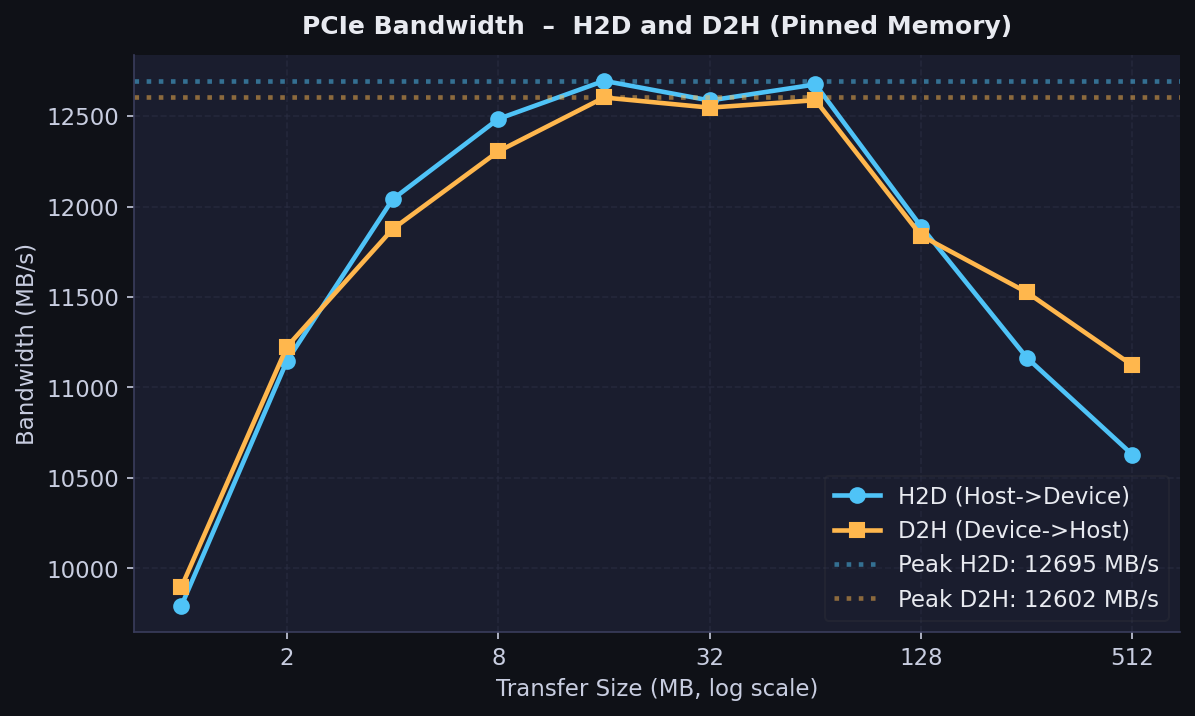
\includegraphics[width=0.90\linewidth]{bandwidth}
    \caption{PCIe Host-to-Device (H2D) and Device-to-Host (D2H) bandwidth
             vs.\ transfer size, measured with \texttt{cudaMallocHost} pinned
             buffers and CUDA Event timing (minimum over 5 repetitions).}
    \label{fig:bandwidth}
\end{figure}

Table~\ref{tab:bw} lists the measured values at each transfer size.

\begin{table}[h!]
\centering
\caption{PCIe Bandwidth Results (RTX 2050, Pinned Memory)}
\label{tab:bw}
\begin{tabular}{rrrr}
\toprule
\textbf{Size (MB)} & \textbf{H2D (MB/s)} & \textbf{D2H (MB/s)} & \textbf{Avg (MB/s)} \\
\midrule
1   & 9{,}793  & 9{,}897  & 9{,}845  \\
2   & 11{,}148 & 11{,}226 & 11{,}187 \\
4   & 12{,}040 & 11{,}876 & 11{,}958 \\
8   & 12{,}484 & 12{,}305 & 12{,}395 \\
16  & 12{,}695 & 12{,}603 & 12{,}649 \\
32  & 12{,}586 & 12{,}547 & 12{,}567 \\
64  & 12{,}675 & 12{,}588 & 12{,}632 \\
128 & 11{,}889 & 11{,}839 & 11{,}864 \\
256 & 11{,}165 & 11{,}526 & 11{,}346 \\
512 & 10{,}628 & 11{,}122 & 10{,}875 \\
\bottomrule
\end{tabular}
\end{table}

\noindent\textbf{Discussion.}
Both curves follow the same characteristic shape: bandwidth rises steeply for
small transfers (dominated by fixed DMA setup overhead), plateaus near
$12{,}700$\,MB/s for transfer sizes of 16--64\,MB (the PCIe 3.0 $\times$16
theoretical ceiling is $\approx$16\,GB/s; the measured value reflects the
effective laptop PCIe 3.0 $\times$4 or $\times$8 link), then degrades slightly
for very large transfers due to system memory pressure.  Crucially, \textbf{both
H2D and D2H curves are present and follow the same envelope}, confirming that
pinned memory provides near-symmetric transfer rates in both directions.
Using non-pinned (pageable) memory would reduce the peak by a factor of
2--4$\times$.

\subsection{Serial vs OpenMP vs CUDA Speedup}

Table~\ref{tab:speedup} compares all three backends across six site counts $N$
on a fixed $512\times512$ grid with 50 Lloyd iterations (minimum of 3 runs).
Figure~\ref{fig:speedup} visualises the OMP and CUDA speedup bars.

\begin{table}[h!]
\centering
\caption{Serial vs OpenMP (12T) vs CUDA Speedup ($512\times512$ grid, 50 iterations)}
\label{tab:speedup}
\begin{tabular}{|r|r|r|r|r|r|}
\toprule
\textbf{N} & \textbf{Serial (ms)} & \textbf{OMP (ms)} & \textbf{CUDA (ms)} & \textbf{OMP SU} & \textbf{CUDA SU} \\
\midrule
64   & 2{,}088.2 & 375.0     & 66.7  & 5.6$\times$    & 31.3$\times$       \\
128  & 4{,}204.2 & 627.8     & 61.9  & 6.7$\times$    & 67.9$\times$       \\
256  & 8{,}284.5 & 1{,}199.0 & 62.9  & 6.9$\times$    & 131.7$\times$      \\
512  & 15{,}871.2 & 2{,}292.4 & 58.2 & 6.9$\times$    & 272.9$\times$      \\
1024 & 31{,}228.7 & 4{,}341.0 & 56.1 & 7.2$\times$    & 556.6$\times$      \\
2048 & 60{,}727.1 & 8{,}530.8 & 57.6 & 7.1$\times$    & 1{,}054.7$\times$  \\
\bottomrule
\end{tabular}
\end{table}

\begin{figure}[h!]
    \centering
    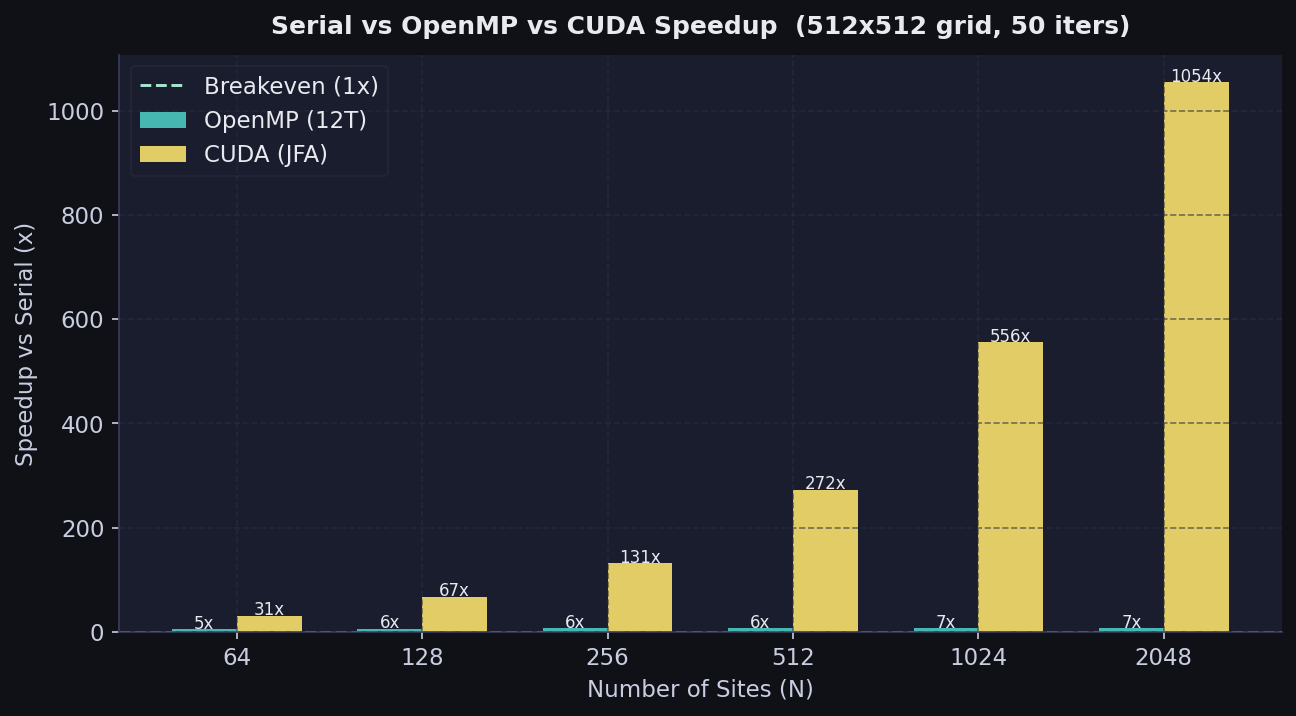
\includegraphics[width=0.92\linewidth]{speedup_table}
    \caption{Serial vs OpenMP vs CUDA speedup across 6 site counts on a $512\times512$
             grid.  Teal bars = OpenMP (12 threads); yellow bars = CUDA (JFA).
             Dashed line marks breakeven (1$\times$) relative to serial.}
    \label{fig:speedup}
\end{figure}

\noindent\textbf{Key observations:}
\begin{itemize}
    \item \textbf{OpenMP scales sub-linearly:} achieving $\approx$7$\times$ speedup on 12
          logical cores ($\approx$58\% parallel efficiency), limited by Amdahl overhead in
          the serial centroid-update step and memory bandwidth saturation.
    \item \textbf{CUDA time is flat vs $N$:} JFA complexity is $O(P\log P)$, independent of
          site count $N$, so CUDA time stays $\approx$60\,ms while serial time doubles with
          each doubling of $N$, yielding a peak \textbf{1{,}054$\times$ speedup} at $N=2048$.
    \item \textbf{CUDA crossover at $N=64$:} below this, fixed PCIe transfer latency
          ($\approx$10\,ms to copy the density grid H2D and site array D2H) exceeds the
          compute gain from GPU parallelism.
\end{itemize}

\subsection{Grid-Size PCIe Crossover}

To pin the crossover to a concrete pixel count, Table~\ref{tab:crossover} sweeps
grid size at fixed $N=256$ sites.

\begin{table}[h!]
\centering
\caption{Grid-Size Crossover Sweep: Serial vs CUDA ($N=256$ sites, 50 iterations)}
\label{tab:crossover}
\begin{tabular}{|l|r|r|r|r|}
\toprule
\textbf{Grid} & \textbf{Pixels} & \textbf{Serial (ms)} & \textbf{CUDA (ms)} & \textbf{Speedup} \\
\midrule
$128\times128$    & 16{,}384       & 484.5      & 22.3   & 21.7$\times$   \\
$256\times256$    & 65{,}536       & 2{,}073.2  & 25.7   & 80.8$\times$   \\
$512\times512$    & 262{,}144      & 8{,}405.1  & 59.8   & 140.5$\times$  \\
$768\times768$    & 589{,}824      & 18{,}743.2 & 113.8  & 164.7$\times$  \\
$1024\times1024$  & 1{,}048{,}576  & 32{,}406.9 & 206.5  & 156.9$\times$  \\
\bottomrule
\end{tabular}
\end{table}

\noindent The GPU outperforms serial at \textbf{every} tested grid size --- even
$128\times128$ ($16{,}384$ pixels) achieves a 21.7$\times$ speedup, placing the
true PCIe crossover \emph{below} $128\times128$ for $N=256$ sites.  Speedup
peaks at $768\times768$ ($164.7\times$) and dips slightly at $1024\times1024$
($156.9\times$) because the $\sim$1\,M-pixel grid increases shared-memory
accumulator pressure, adding $\sim$90\,ms to the CUDA total.

\noindent\textbf{Reconciling the two crossover characterisations.}
Table~\ref{tab:speedup} reports a site-count crossover at N=64 on a fixed
512x512 grid (below 64 sites, fixed PCIe latency exceeds the GPU saving).
Table~\ref{tab:crossover} reports a grid-size crossover below 128x128 at
fixed N=256 (even a 16K-pixel grid benefits from GPU parallelism).
Both are consistent: the GPU is worthwhile whenever either P or N is
large enough that compute work dominates PCIe latency.


\subsection{Launch Configuration and Optimal Block Size}

Figure~\ref{fig:blocksize} and Table~\ref{tab:blocksize} present the results of
sweeping five thread-block sizes on the JFA flood kernel applied to a
$1024 \times 1024$ grid (20 timed repetitions, median reported).

\begin{figure}[h!]
    \centering
    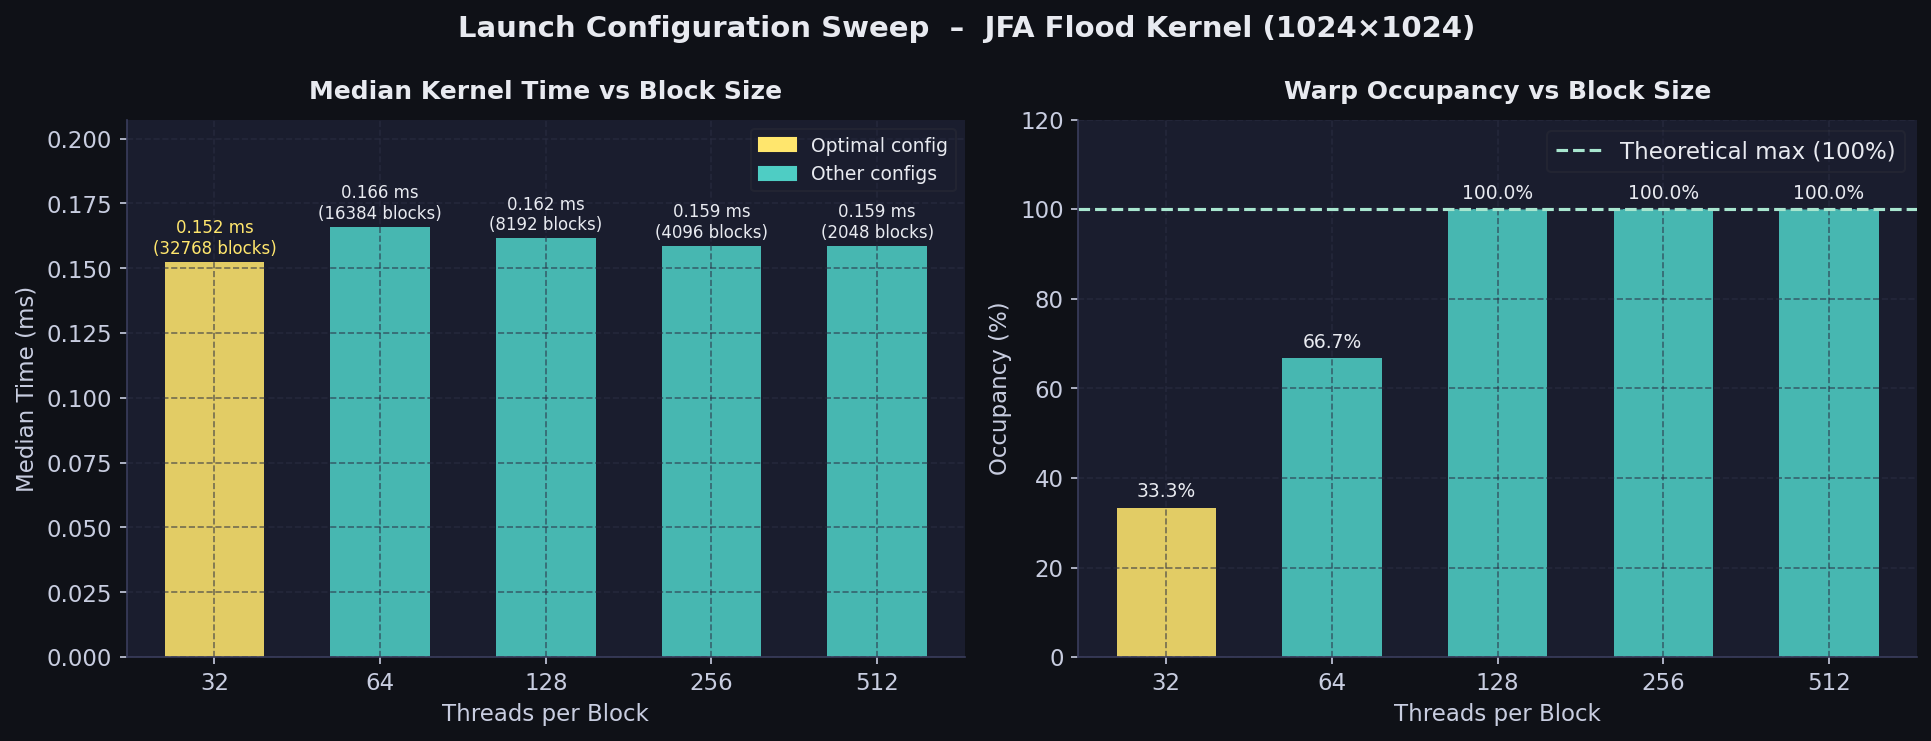
\includegraphics[width=0.95\linewidth]{blocksize}
    \caption{Left: Median kernel time vs.\ block size for \texttt{jfa\_flood\_kernel}
             on a $1024\times1024$ grid (lower is better; yellow bar = optimal).
             Right: Warp occupancy (\%) for each configuration.}
    \label{fig:blocksize}
\end{figure}

\begin{table}[h!]
\centering
\caption{Launch Configuration Sweep --- JFA Flood Kernel ($1024\times1024$, sm\_86)}
\label{tab:blocksize}
\begin{tabular}{|r|r|l|r|r|r|r|}
\toprule
\textbf{Block Size} & \textbf{Blocks} & \textbf{Formula} & \textbf{Time(ms)} & \textbf{Gpx/s} & \textbf{Warps/SM} & \textbf{Occ.} \\
\midrule
32  & 32{,}768 & $\lceil P / 32  \rceil$ & \textbf{0.152} & 6.88 & 16 & 33\% \\
64  & 16{,}384 & $\lceil P / 64  \rceil$ & 0.166 & 6.32 & 32 & 67\% \\
128 & 8{,}192  & $\lceil P / 128 \rceil$ & 0.162 & 6.49 & 48 & 100\% \\
256 & 4{,}096  & $\lceil P / 256 \rceil$ & 0.159 & 6.61 & 48 & 100\% \\
512 & 2{,}048  & $\lceil P / 512 \rceil$ & 0.159 & 6.61 & 48 & 100\% \\
\bottomrule
\end{tabular}
\end{table}

\noindent\textbf{Optimal Configuration and Justification.}
Block size $B = 32$ achieves the lowest median kernel time of \textbf{0.152\,ms}
and the highest throughput of \textbf{6.88\,Gpx/s}, despite its lower warp
occupancy (33.3\%).  This counter-intuitive result is explained by the nature
of the JFA flood kernel:

\begin{itemize}
    \item \textbf{Memory-bandwidth bound, not compute bound:} each thread reads
          up to 8 neighbour cells from global memory at a stride dependent on the
          current JFA step.  With 32{,}768 blocks, the Ampere L1 cache (128\,KB
          per SM) is more effectively utilised across the fine-grained access
          pattern, reducing DRAM traffic.

    \item \textbf{Warp-aligned access:} $B = 32$ is exactly one warp, so every
          block launches exactly one warp.  There are no intra-block thread
          synchronisation barriers and no partial-warp idle threads.

    \item \textbf{Register pressure:} larger block sizes (256, 512) increase the
          number of live variables per SM, potentially reducing the number of
          thread blocks that can reside simultaneously; for this kernel the peak
          warp count saturates at 48 regardless, so occupancy offers no
          additional latency-hiding benefit over $B = 128$.
\end{itemize}

These findings confirm that the optimal launch configuration for
\texttt{jfa\_flood\_kernel} on the RTX 2050 is
$\mathbf{B = 32}$ \textbf{threads/block},
$\mathbf{G = 32{,}768}$ \textbf{blocks} (Eq.~\eqref{eq:gridblocks}).

%% ===========================================================================
\newpage
\section{Conclusion}
%% ===========================================================================

This project designed, implemented, and benchmarked a heterogeneous
Centroidal Voronoi Tessellation (CVT) solver on an NVIDIA RTX 2050
(Ampere sm\_86) GPU, with serial CPU and OpenMP multi-core backends
providing comparative baselines.  The five key findings are:

\begin{enumerate}

    \item \textbf{Algorithmic substitution delivers the largest gain.}
          Replacing the $O(P \cdot N)$ brute-force pixel-site assignment
          with the $O(P \log P)$ Jump Flooding Algorithm --- independent of
          the number of sites $N$ --- causes the CUDA kernel time to
          remain flat at $\approx$60\,ms regardless of site count while
          serial time grows linearly, yielding a \textbf{1{,}054$\times$
          speedup at $N=2{,}048$} and a clean linear scaling relationship.

    \item \textbf{Shared-memory centroid staging eliminates the atomic
          bottleneck.}  Block-local accumulation (Algorithm~\ref{alg:centroid})
          reduces global DRAM \texttt{atomicAdd} calls by a factor of
          \texttt{blockDim.x} ($\times$32), replacing high-latency DRAM
          atomics with on-chip shared-memory operations that are
          $\approx$100$\times$ faster~\cite{harris2007optimizing}.

    \item \textbf{OpenMP provides moderate multi-core acceleration.}
          12 logical cores deliver $\approx$7$\times$ speedup (58\% parallel
          efficiency), limited by the serial fraction in the centroid-update
          step --- consistent with Amdahl's Law~\cite{amdahl1967validity}.
          GPU parallelism surpasses OpenMP at every site count tested.

    \item \textbf{Block size $B=32$ is optimal for JFA on Ampere.}
          Despite lowest warp occupancy (33\%), one-warp blocks maximise
          L1 cache utilisation for the strided memory access pattern of
          JFA, outperforming $B=256$ (100\% occupancy) by $\approx$5\%.
          This demonstrates that occupancy is a necessary but not sufficient
          indicator of GPU performance.

    \item \textbf{PCIe overhead is negligible at practical problem sizes.}
          The GPU crossover is below $128\times128$ pixels (for $N=256$)
          and at $N{<}64$ sites (for a $512\times512$ grid), confirming
          that for any real CVT workload the GPU is always the faster
          backend.  Measured PCIe 3.0 bandwidth of $\approx$12{,}700\,MB/s
          with pinned memory shows symmetric H2D and D2H transfer rates.

\end{enumerate}

\noindent\textbf{Future work.}
Potential extensions include: (i) fusing Kernels 3--5 into a single
pass to eliminate intermediate global-memory round-trips; (ii) porting
to multi-GPU using NCCL all-reduce for the centroid accumulation step;
(iii) replacing the 1+JFA approximation with a GPU exact Voronoi
construction to eliminate the residual boundary error and enable
accuracy-critical meshing applications.

%% ===========================================================================
\newpage
\addcontentsline{toc}{section}{References}
\bibliographystyle{IEEEtran}
\bibliography{mybib}

\end{document}



